%% ============================================================
%%  CHAPTER 11 — CONFIGURATION AND CONTROL APPLICATION
%% ============================================================
\chapter{Configuration and Control Application}
\label{ch:application}

This chapter describes the application layer that sits between the
classifier output (Chapter~9, deployed in real time in Chapter~12)
and the physical prosthetic hand (Chapter~4): the ESP32 firmware
that receives classified gestures, drives the servos, and hosts a
fully offline configuration web app over its own WiFi network.
Section~\ref{sec:app_overview} positions this layer in the overall
system and introduces the two interface contracts that govern it.
Section~\ref{sec:app_build} describes the layered firmware build
plan and its current implementation status.
Section~\ref{sec:app_contracta} specifies Contract~A, the
\acrshort{uart} interface between the classifier host and the
ESP32. Section~\ref{sec:app_contractb} specifies Contract~B, the
\acrshort{rest} and WebSocket web API the ESP32 serves to the
browser. Section~\ref{sec:app_datamodels} defines the mapping and
pose data models shared by both firmware and web app.
Section~\ref{sec:app_failsafe} describes the fail-safe behaviour.
Section~\ref{sec:app_webapp} describes the offline web application
itself --- its design, its three screens, the 3D digital twin, and
its mock-mode architecture. Section~\ref{sec:app_status} reports
the honest implementation status of every layer at the time of
writing. Section~\ref{sec:app_summary} summarises the chapter.

%% ----------------------------------------------------------
\section{System Position and the Two Contracts}
\label{sec:app_overview}
%% ----------------------------------------------------------

As established in Chapter~4, the deployed system is a three-node
distributed pipeline:

\begin{center}
EEG headset $\rightarrow$ Raspberry Pi 5 (classifier, Chapter~12)
$\xrightarrow{\text{\acrshort{uart}}}$ ESP32 (this chapter)
$\xrightarrow{\text{WiFi AP}}$ phone / laptop (this chapter)
\end{center}

The ESP32 firmware, and the web application it serves, are governed
by exactly two interface contracts, deliberately kept small and
mirrored in code (\code{include/contracts.h}) so that firmware and
web app cannot silently drift apart:

\begin{itemize}[leftmargin=*]
    \item \textbf{Contract A} (Section~\ref{sec:app_contracta}) ---
    the \acrshort{uart} message format by which the classifier host
    (Raspberry Pi, running the real-time inference pipeline of
    Chapter~12) sends gesture labels to the ESP32.
    \item \textbf{Contract B} (Section~\ref{sec:app_contractb}) ---
    the \acrshort{rest} and WebSocket API by which the ESP32 serves
    a configuration dashboard to any phone or laptop joined to its
    WiFi access point.
\end{itemize}

Everything else in this chapter --- the mapping editor, the pose
creator, the 3D digital twin --- is built on top of these two
contracts and does not introduce any additional interface surface.

%% ----------------------------------------------------------
\section{Firmware Build Plan}
\label{sec:app_build}
%% ----------------------------------------------------------

The firmware is developed in deliberate, independently verifiable
layers rather than as a single monolithic build, so that each layer
can be flashed and boot-tested on real hardware before the next is
attempted. Table~\ref{tab:build_layers} lists the six layers.

\begin{table}[htbp]
\centering
\caption{Firmware build layers. Status reflects the state at the
time of writing (Section~\ref{sec:app_status} discusses the
implications of this in full).}
\label{tab:build_layers}
\renewcommand{\arraystretch}{1.3}
\begin{tabular}{c p{7.5cm} c}
\toprule
\textbf{Layer} & \textbf{Scope} & \textbf{Status} \\
\midrule
0 & Scaffold: \code{platformio.ini}, both contracts, default
    \code{mappings.json}/\code{poses.json}, filesystem self-heal &
    \ding{51} Done --- flashed and boot-verified on hardware \\
1 & PCA9685 servo core, built-in actions, \acrshort{uart} listener,
    fail-safe & Next \\
2 & WiFi access point, read-only status dashboard, WebSocket &
    Not started \\
3 & Mapping editor (remap labels live) & Not started \\
4 & Pose creator (sliders drive the real hand; save/apply/delete)
    & Not started \\
5 & Three.js 3D digital twin (stretch goal; degrades gracefully) &
    Not started \\
\bottomrule
\end{tabular}
\end{table}

Layer~0 is the only layer verified on physical hardware at the time
of writing: the boot banner prints over serial at 115200 baud,
LittleFS mounts, both default JSON configuration files load (or are
auto-created if missing), and both contracts parse correctly (7
valid labels, 7 built-in actions, 1 default saved pose). Flash
footprint on the 4\,MB target board is approximately 16\%
($\approx$319\,KB), leaving ample headroom for Layers~1--5.

\subsection{Build Configuration}

The firmware targets two build environments defined in
\code{platformio.ini}: a primary 8\,MB-flash environment
(\code{esp32dev}, with a custom \code{partitions\_8mb.csv}
allocating $\approx$3\,MB to the application and $\approx$4.8\,MB to
the LittleFS data partition that stores the web app assets and JSON
configuration), and a 4\,MB fallback environment
(\code{esp32dev\_4mb}) for the specific board actually mounted in
the hand, which has 4\,MB of flash rather than the originally
targeted 8\,MB. All hardware pin assignments, WiFi credentials, and
system timeouts are centralised in a single header,
\code{include/config.h}, so that adapting the firmware to different
wiring requires editing exactly one file.

%% ----------------------------------------------------------
\section{Contract A: UART Interface (Pi $\rightarrow$ ESP32)}
\label{sec:app_contracta}
%% ----------------------------------------------------------

\subsection{Physical Link and Message Format}

The classifier host and the ESP32 communicate over the ESP32's
\code{Serial2} hardware \acrshort{uart}, wired Pi TX
$\rightarrow$ ESP32 GPIO16 (RX) and Pi RX $\leftarrow$ ESP32 GPIO17
(TX), with a common ground, at 115200 baud, 8N1 --- the same link
described from the classifier host's side in Chapter~4. The
protocol is deliberately minimal: the Pi sends one
\code{lowercase\_snake\_case} label per line, newline-terminated
ASCII (e.g.\ \code{clinch\textbackslash n}). The ESP32 parses each
line, looks the label up in the current mapping table
(Section~\ref{sec:app_datamodels}), and executes the resulting
action. \textbf{Unknown labels are logged and ignored} --- the
firmware never crashes and never moves the hand in response to an
unrecognised label, which is an intentional fail-closed design
choice given that a misinterpreted UART line driving an unintended
servo motion would be a safety concern for a hand near a user's
face.

\subsection{Valid Labels: A Known Inconsistency}
\label{sec:app_label_mismatch}

The valid-label set currently defined in \code{include/contracts.h}
and mirrored in the default \code{mappings.json} is a
\textbf{seven-label placeholder scaffold} --- \code{eye\_blink},
\code{double\_blink}, \code{jaw\_clench}, \code{eyebrow\_raise},
\code{look\_left}, \code{look\_right}, and \code{rest} --- carried
over from an earlier, more generic phase of the firmware design,
before the final classifier taxonomy (Chapter~6) was locked in.
\textbf{This does not match the five labels the production
classifier actually emits}
(\code{single\_blink}, \code{double\_blink}, \code{clinch},
\code{bruxism\_left}, \code{bruxism\_right}). Two of the seven
placeholder labels have no classifier counterpart at all
(\code{eyebrow\_raise}, \code{look\_left}, \code{look\_right} ---
gestures that were never part of the final 5-class taxonomy;
Chapter~6), and one classifier label has no placeholder counterpart
(\code{single\_blink}, currently only representable via the
generic \code{eye\_blink}).

This is flagged here explicitly, rather than silently reconciled,
because it is a genuine open item: \code{contracts.h} and the
default \code{mappings.json} need to be updated to the real
five-label set before Layer~1 (\acrshort{uart} listener) is
built, or the firmware will be listening for labels the classifier
will never send. Table~\ref{tab:label_reconciliation} gives the
intended final mapping, which \textbf{this report treats as
authoritative going forward} even though it is not yet reflected in
the shipped configuration files.

\begin{table}[htbp]
\centering
\caption{Intended final label $\rightarrow$ built-in action mapping,
reconciling the classifier's real output labels (Chapter~6) with
the firmware's built-in actions (Section~\ref{sec:app_datamodels}).
This supersedes the placeholder seven-label scaffold currently
shipped in \code{contracts.h}.}
\label{tab:label_reconciliation}
\renewcommand{\arraystretch}{1.3}
\begin{tabular}{l l l}
\toprule
\textbf{Classifier label} & \textbf{Command} & \textbf{Action} \\
\midrule
\code{single\_blink}  & O & \code{open\_hand} \\
\code{double\_blink}  & S & \code{pinch} \\
\code{clinch}         & C & \code{close\_fist} \\
\code{bruxism\_left}  & L & \code{wrist\_left} \\
\code{bruxism\_right} & R & \code{wrist\_right} \\
\bottomrule
\end{tabular}
\end{table}

Because the mapping table is user-editable at runtime
(Section~\ref{sec:app_contractb}), this reconciliation does not
require a firmware rebuild once Layer~3 (the mapping editor) is in
place --- only the \emph{default} shipped mapping needs to change;
a user could otherwise remap any label to any action at any time
through the web app.

%% ----------------------------------------------------------
\section{Contract B: Web API (ESP32 $\rightarrow$ Browser)}
\label{sec:app_contractb}
%% ----------------------------------------------------------

Once Layer~2 is built, the ESP32 will host a WiFi access point that
the phone or laptop joins directly --- there is no internet
connection at any point in this link, so every asset the browser
loads (HTML, CSS, JavaScript, the 3D model, and the vendored
Three.js library) is served locally from the on-chip LittleFS
filesystem. No content delivery network is used anywhere in the
design, since one would be unreachable without internet access.
Table~\ref{tab:contract_b} lists the complete Contract~B surface.

\begin{table}[htbp]
\centering
\caption{Contract B: the complete REST and WebSocket surface served
by the ESP32.}
\label{tab:contract_b}
\renewcommand{\arraystretch}{1.3}
\begin{tabular}{l l p{6.0cm}}
\toprule
\textbf{Method} & \textbf{Path} & \textbf{Purpose} \\
\midrule
GET    & \code{/}                 & The web app (\code{index.html}) \\
GET    & \code{/api/status}       & Live status snapshot \\
GET    & \code{/api/mappings}     & Current label $\rightarrow$ action map \\
POST   & \code{/api/mappings}     & Replace/update the map (persisted to LittleFS) \\
GET    & \code{/api/poses}        & List of saved poses \\
POST   & \code{/api/poses}        & Create/update a named pose (persisted) \\
DELETE & \code{/api/poses/\{name\}} & Delete a pose \\
POST   & \code{/api/servo}        & Live-set one servo angle (pose-editor preview) \\
POST   & \code{/api/pose/apply}   & Apply a saved pose by name immediately \\
POST   & \code{/api/relax}        & Emergency open/relax \\
WS     & \code{/ws}                & Push live status at 5--10\,Hz (no polling) \\
\bottomrule
\end{tabular}
\end{table}

\subsection{Request and Response Shapes}

\begin{lstlisting}[language=json,
    caption={\code{GET /api/status} response --- also the shape
    pushed periodically over the \code{/ws} WebSocket.},
    label={lst:api_status}]
{
  "battery_pct": 87,
  "battery_v": 7.92,
  "linkA_connected": true,
  "last_label": "clinch",
  "last_label_ms_ago": 412,
  "servo_angles": [120, 100, 10, 10, 10, 90],
  "active_pose": "close_fist",
  "failsafe": false
}
\end{lstlisting}

\begin{lstlisting}[language=json,
    caption={\code{POST /api/mappings} request body --- the server
    replaces the stored map wholesale and persists it.},
    label={lst:api_mappings}]
{ "clinch": "close_fist", "double_blink": "pinch", "...": "..." }
\end{lstlisting}

\begin{lstlisting}[language=json,
    caption={\code{POST /api/poses} request body.},
    label={lst:api_poses}]
{ "name": "ok_sign", "angles": [120, 100, 10, 10, 10, 90] }
\end{lstlisting}

\begin{lstlisting}[language=json,
    caption={\code{POST /api/servo} request body --- used by the
    pose editor's sliders to preview one joint at a time on the
    real hand.},
    label={lst:api_servo}]
{ "channel": 1, "angle": 95 }
\end{lstlisting}

\begin{lstlisting}[language=json,
    caption={\code{POST /api/pose/apply} request body.},
    label={lst:api_apply}]
{ "name": "pinch" }
\end{lstlisting}

The WebSocket endpoint (\code{/ws}) exists specifically to avoid
polling: rather than the browser repeatedly issuing
\code{GET~/api/status} requests, the ESP32 pushes the same status
shape (Listing~\ref{lst:api_status}) to every connected client every
\code{WS\_PUSH\_INTERVAL\_MS} (5--10\,Hz), which is both lower
overhead for the microcontroller and gives the web app's live
telemetry --- battery level, last received label, and current servo
angles --- a smoother, near-real-time feel.

%% ----------------------------------------------------------
\section{Data Models}
\label{sec:app_datamodels}
%% ----------------------------------------------------------

\subsection{Mapping (\code{mappings.json})}

A mapping is a flat JSON object where each valid label maps to an
\textbf{action string}, and an action string is either one of the
seven built-in actions or the name of a user-saved pose:

\begin{lstlisting}[language=json,
    caption={Mapping data model.}, label={lst:mapping_model}]
{ "clinch": "close_fist", "double_blink": "pinch" }
\end{lstlisting}

\subsection{Pose (\code{poses.json})}

A pose is a named, fixed set of joint angles:

\begin{lstlisting}[language=json,
    caption={Pose data model. \texttt{angles} always has exactly 6
    entries, 0--180 degrees, in channel order.},
    label={lst:pose_model}]
{ "poses": [
    { "name": "pinch", "angles": [a0, a1, a2, a3, a4, a5] }
] }
\end{lstlisting}

\noindent where the six angles are in the fixed channel order
established in Chapter~4: \code{[thumb, index, middle, ring,
pinky, wrist]}, matching PCA9685 channels 0--5.

\subsection{Built-In Actions}

Seven actions are implemented directly in firmware and are always
valid as a mapping target, in addition to any saved pose name:
\code{open\_hand}, \code{close\_fist}, \code{point}, \code{pinch},
\code{wrist\_left}, \code{wrist\_right}, and \code{relax}. This
means the mapping table has two tiers of indirection: a label maps
to \emph{either} a hard-coded built-in action \emph{or} a
user-defined pose, and the firmware does not need to distinguish
between the two cases when executing a mapped action --- both are
simply a target set of six joint angles.

%% ----------------------------------------------------------
\section{Fail-Safe Behaviour}
\label{sec:app_failsafe}
%% ----------------------------------------------------------

If no valid label arrives over Contract~A within
\code{FAILSAFE\_TIMEOUT\_MS} (default 3{,}000\,ms), the hand
\textbf{holds its current position} rather than going limp or
snapping to a default pose. This design choice matters
practically: a prosthetic hand that suddenly relaxed every time the
classifier briefly failed to detect a gesture (for example, during
a rest period between commands, which is the expected, common case
--- not an error state) would be unusable, releasing whatever the
user was holding. Holding position on timeout treats the absence of
a new command as ``no change requested,'' not as an error. A manual
escape hatch is still provided: \code{POST /api/relax} is exposed
in the web app as an explicit emergency open/relax button for the
cases where the user does want to release deliberately.

%% ----------------------------------------------------------
\section{The Web Application}
\label{sec:app_webapp}
%% ----------------------------------------------------------

\subsection{Design Goals}

The web app is a vanilla-JavaScript single-page application ---
no framework, no build step, no CDN dependency of any kind ---
living entirely in the firmware's \code{data/} directory (the
LittleFS image). It is explicitly designed to feel like a
\textbf{native phone app} rather than a web page when opened on the
phone that has joined the ESP32's access point: full-screen layout,
a phone-frame presentation when viewed on a desktop browser, and a
bottom tab bar with three sections (Home, Mappings, Poses). The
visual theme is deliberately described as ``light clinical'' ---
white and blue, rounded cards, mobile-first --- appropriate to a
medical/assistive-device configuration tool used one-handed on a
phone.

\subsection{Home: The 3D Digital Twin}

The Home screen centres on a drag-to-rotate 3D model of the InMoov
hand, rendered with real WebGL via a locally vendored copy of
Three.js r137 (no external script tags, consistent with the no-CDN
requirement). \code{hand3d.js} loads a GLB model
(\code{models/hand.glb}) if present, and falls back to a
procedurally generated articulated robot hand if the model file is
missing --- so the 3D view degrades gracefully rather than failing
outright on a fresh or minimal filesystem image. The digital twin
re-poses live as gesture cues arrive (via the WebSocket push of
\code{servo\_angles}, Listing~\ref{lst:api_status}), giving the user
a visual confirmation of what the physical hand is doing without
needing to look directly at it. Figure~\ref{fig:webapp_home} shows
this screen running in mock mode.

\begin{figure}[htbp]
\centering
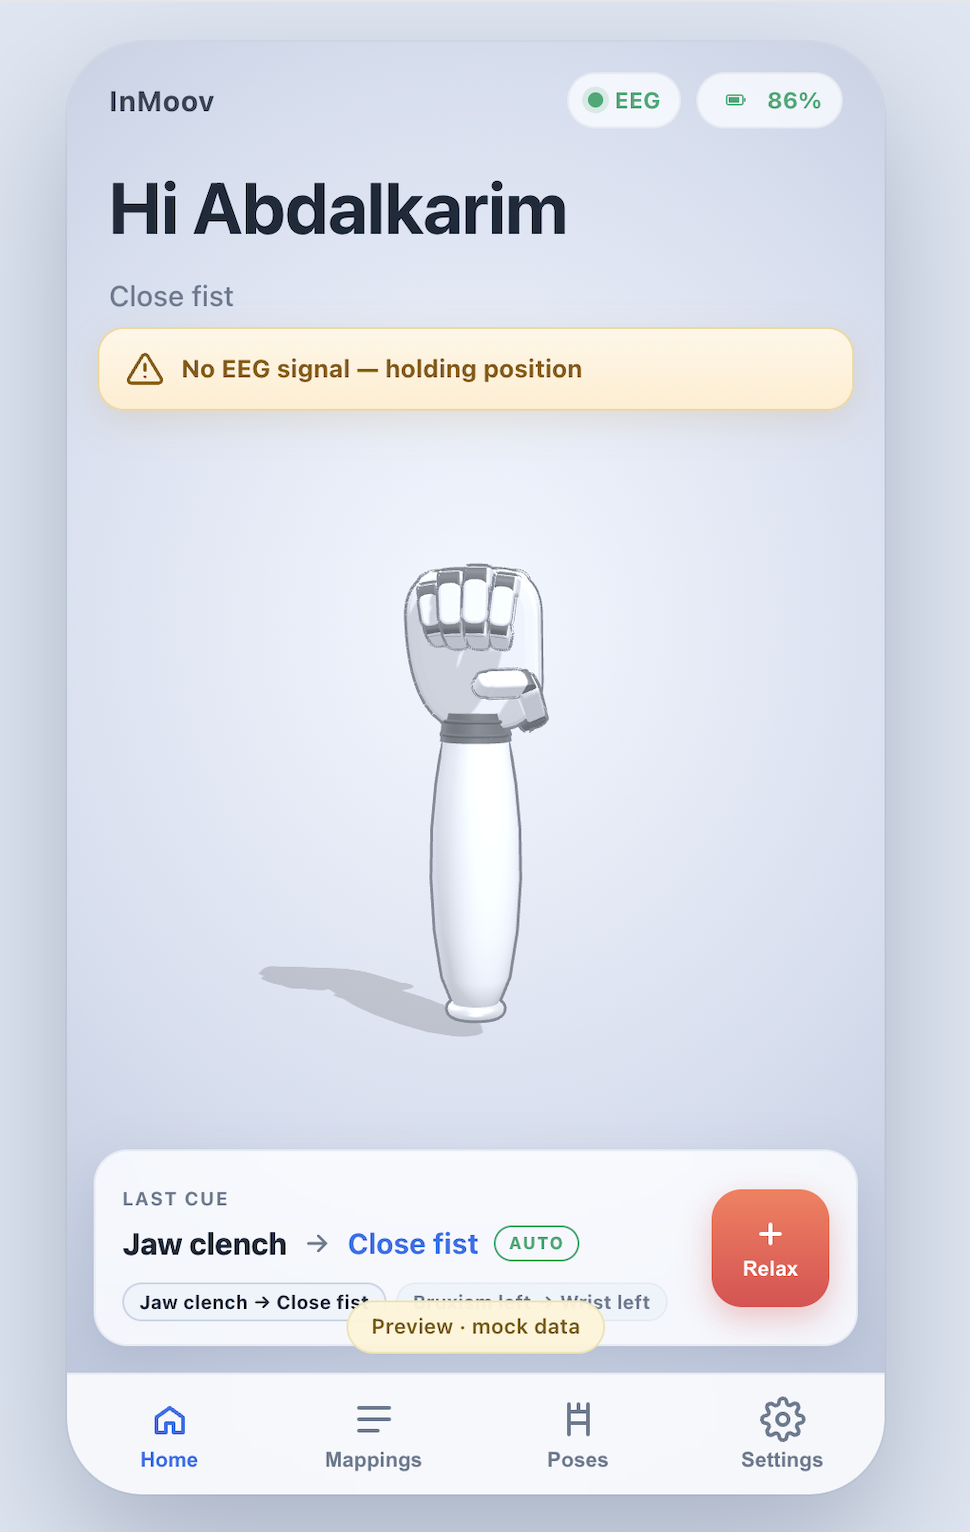
\includegraphics[width=0.4\textwidth]{Assets/webapp_home_3d}
\caption{Home screen of the configuration web application: a
drag-to-rotate WebGL model of the InMoov hand (the ``digital twin'')
that re-poses live as gesture cues arrive, shown here in mock mode.}
\label{fig:webapp_home}
\end{figure}

\subsection{Mappings and Poses Editors}

The Mappings and Poses screens are thin editors over the Contract~B
REST endpoints described in Section~\ref{sec:app_contractb}: the
Mappings screen lists every valid label next to a selector for its
current action (built-in or saved pose) and issues
\code{POST~/api/mappings} on save; the Poses screen exposes six
sliders (one per servo channel) that drive \code{POST~/api/servo}
live for immediate visual and physical feedback while editing, plus
save/apply/delete controls that call \code{POST~/api/poses},
\code{POST~/api/pose/apply}, and \code{DELETE~/api/poses/\{name\}}
respectively. A lightweight inline \acrshort{svg} hand diagram
mirrors the slider values as a simplified 2D preview alongside the
3D twin, so the pose editor remains usable even in the procedural-fallback
case where no GLB model is present. The two editors are shown in
Figure~\ref{fig:webapp_editors}.

\begin{figure}[htbp]
\centering
\begin{subfigure}[t]{0.46\textwidth}
\centering
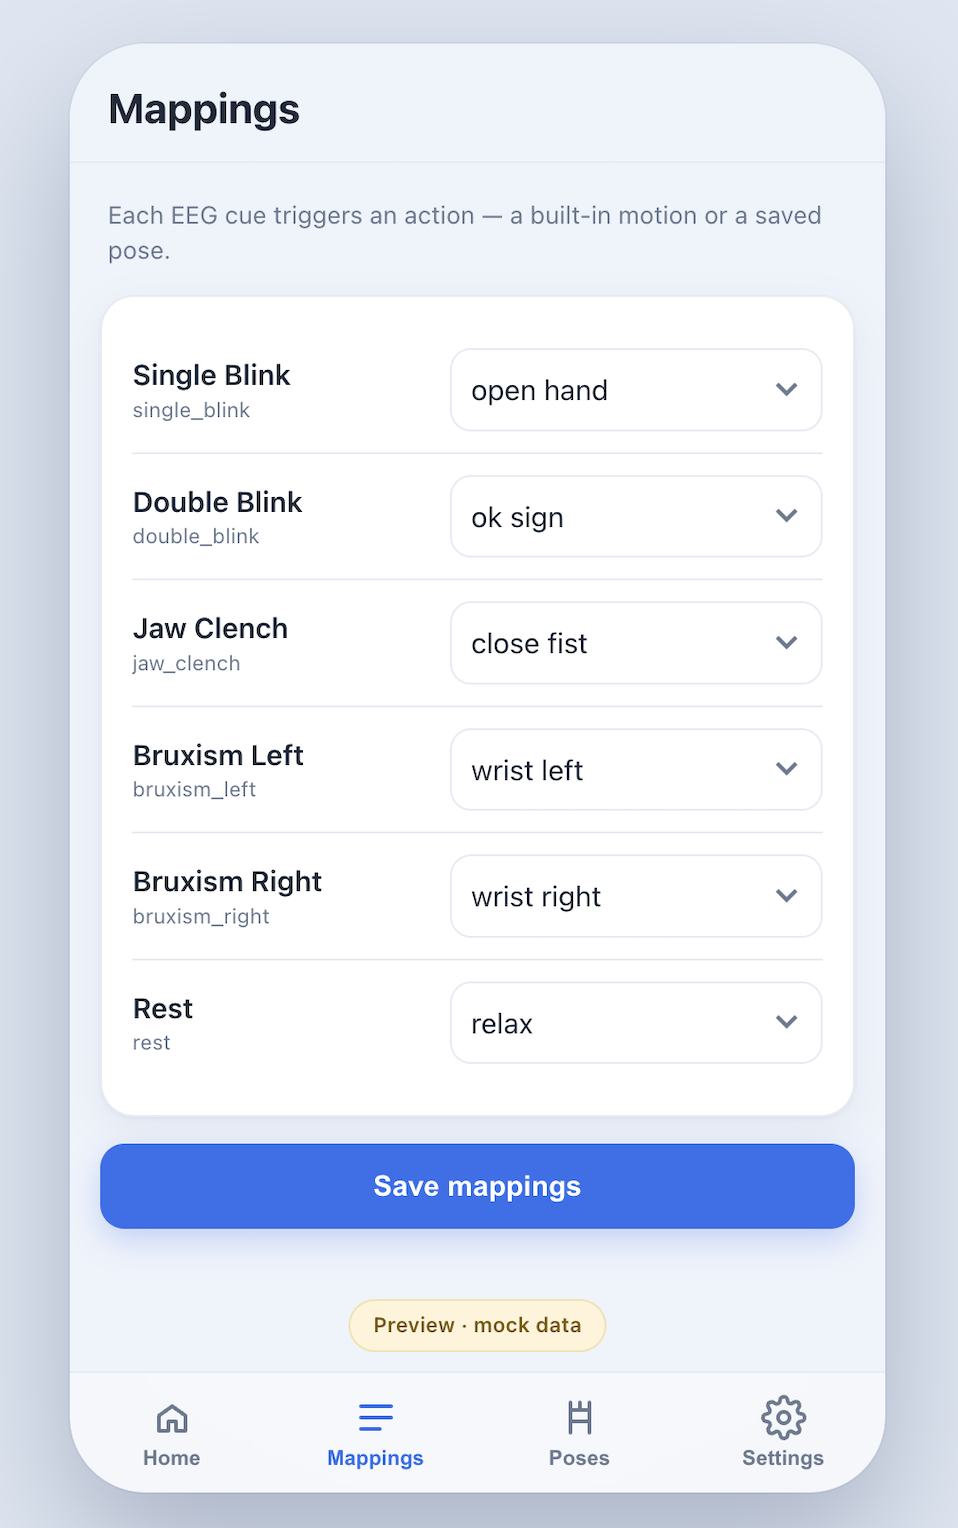
\includegraphics[width=\textwidth]{Assets/webapp_mappings}
\caption{Mappings editor}
\label{fig:webapp_mappings}
\end{subfigure}
\hfill
\begin{subfigure}[t]{0.46\textwidth}
\centering
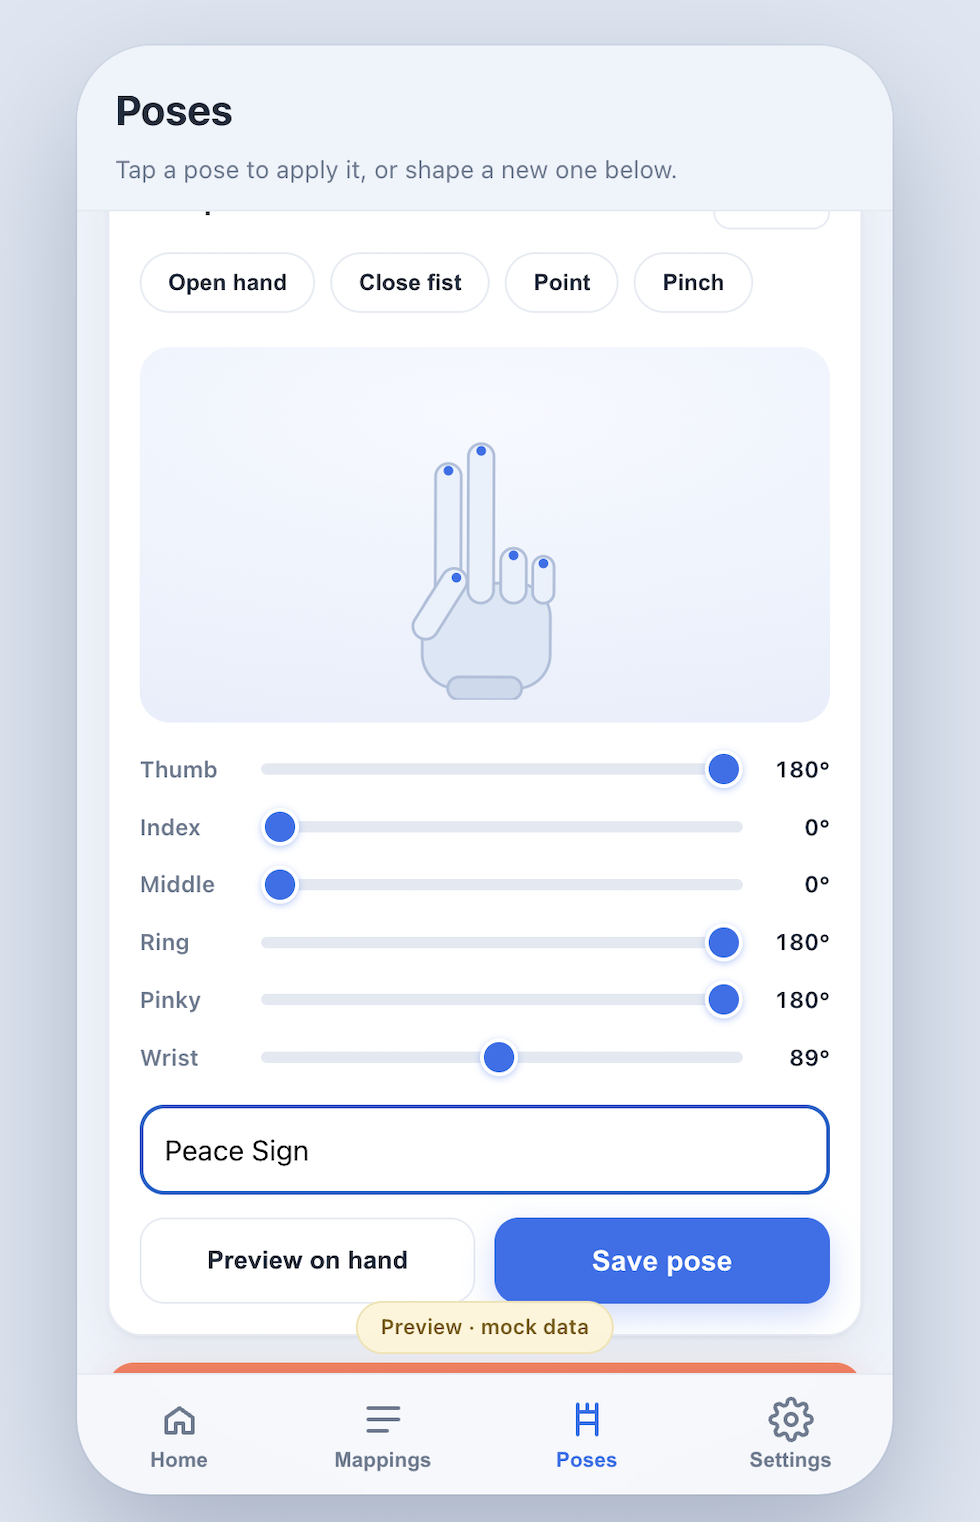
\includegraphics[width=\textwidth]{Assets/webapp_poses}
\caption{Poses editor}
\label{fig:webapp_poses}
\end{subfigure}
\caption{The two configuration editors, running in mock mode.
(a)~The Mappings screen assigns each command label to a built-in
action or a saved pose. (b)~The Poses screen exposes one slider per
servo channel with a live 2D hand preview and save/preview controls.}
\label{fig:webapp_editors}
\end{figure}

\subsection{Mock Mode}
\label{sec:app_mock}

Because the firmware layers that actually serve this web app over
the AP (Layers~2--4, Section~\ref{sec:app_build}) are not yet built,
the web app includes a \textbf{mock mode} so that its design and
interaction flow can be evaluated and iterated on independently of
firmware progress. \code{app.js} auto-detects three conditions ---
the page being opened via the \code{file://} scheme, opened on
\code{localhost}, or opened with a \code{?mock} query parameter ---
and, if any hold, transparently substitutes a simulated
\code{api} object that returns fake status data and simulates an
incoming EEG cue stream, rather than issuing real
\code{fetch}/WebSocket calls. Critically, this simulated \code{api}
object exposes the \emph{same} interface as the real one, so the
same UI code path runs in both mock and live mode: the same object
is where the real \code{/api/*} and \code{/ws} calls will be wired
in once Layers~2+ exist, with no UI-layer changes anticipated at
that point. This is also why the web app can currently be previewed
standalone with \code{python3~-m~http.server} (needed because GLB
model loading requires an HTTP context, which \code{file://} alone
does not reliably provide in all browsers) without any ESP32
hardware attached at all.

\subsection{Planned but Not Yet Implemented: Sequences}

An earlier planning document for the phone app (predating the
Contract~A/B design in this chapter) listed \textbf{saved gesture
sequences} --- chaining multiple poses together, for example, as a
planned feature alongside per-finger control and custom gestures.
This does not currently exist anywhere in Contract~B: there is no
\code{/api/sequences} endpoint, and the pose data model
(Section~\ref{sec:app_datamodels}) has no notion of an ordered
sequence of poses, only single, static poses. It is documented here
explicitly, as a planned-but-unimplemented feature, so that it is
not mistaken for a built capability, and is carried forward as a
concrete future-work item in Chapter~14 rather than silently
dropped.

%% ----------------------------------------------------------
\section{Implementation Status}
\label{sec:app_status}
%% ----------------------------------------------------------

In the interest of the same honesty this report has applied to the
classification methodology (Chapters~6--10), it is worth being
explicit about what is and is not actually running at the time of
writing:

\begin{itemize}[leftmargin=*]
    \item \textbf{Verified on hardware:} Layer~0 only --- the
    firmware scaffold, both contracts parsing correctly, and
    LittleFS serving the default JSON configuration files. This has
    been flashed to the physical ESP32 mounted in the hand and its
    boot banner confirmed over serial.
    \item \textbf{Designed but not yet running on the device:}
    Layers~1--4 (servo control, WiFi access point, mapping editor,
    pose creator) and the web application described in
    Section~\ref{sec:app_webapp}. The web app exists as a complete,
    working prototype, but today it only runs in mock mode
    (Section~\ref{sec:app_webapp}) --- it has not yet been served
    live by the ESP32 over its access point, because the firmware
    layers that would do so are not built.
    \item \textbf{Stretch goal:} Layer~5, the Three.js digital
    twin, is explicitly scoped to degrade gracefully (procedural
    fallback hand) if not completed or if the GLB asset is missing.
    \item \textbf{Known open item:} the Contract~A label mismatch
    (Section~\ref{sec:app_label_mismatch}) must be resolved --- the
    shipped \code{contracts.h} and default \code{mappings.json}
    updated to the real five-label classifier output --- before
    Layer~1 is built, or the \acrshort{uart} listener will be
    listening for labels the classifier will never emit.
\end{itemize}

A stand-in tool, \code{tools/fake\_pi.py}, sends synthetic labels
over serial in place of the real classifier host, allowing Contract~A
and the servo/mapping logic to be exercised and debugged before
the full real-time inference pipeline of Chapter~12 is connected.

%% ----------------------------------------------------------
\section{Chapter Summary}
\label{sec:app_summary}
%% ----------------------------------------------------------

This chapter described the configuration and control application
layer that connects the classifier (Chapter~9, deployed in
real time in Chapter~12) to the physical prosthetic hand
(Chapter~4). Two small, code-mirrored interface contracts govern
the entire layer: Contract~A, a minimal newline-delimited
\acrshort{uart} label protocol from the classifier host to the
ESP32, and Contract~B, a \acrshort{rest} and WebSocket web API
served entirely offline from the ESP32's own WiFi access point,
with no CDN or internet dependency anywhere in the design. A
significant, previously undocumented inconsistency was identified
and flagged: the currently shipped Contract~A label set is a
seven-label generic placeholder that does not match the classifier's
real five-label output, and an authoritative reconciled mapping
table was provided to replace it before Layer~1 is built. The
offline web application --- a vanilla-JavaScript single-page app
with a 3D digital-twin home screen, live mapping and pose editors,
and a mock-mode architecture that lets the entire UI be developed
and evaluated without any ESP32 hardware attached --- was described
in full, along with an explicit, honest statement of implementation
status: only the firmware scaffold (Layer~0) is currently verified
on hardware, with servo control, the WiFi access point, and the
live editors still to be built. A planned ``saved sequences''
feature was identified as not yet part of Contract~B and carried
forward to Chapter~14 as future work. The following chapter
describes the real-time inference pipeline that produces the
Contract~A labels this chapter's firmware consumes.